\documentclass[11pt,a4paper,dvipdfmx]{bxjsarticle}

% --- パッケージのインクルード ---
\usepackage[dvipdfmx]{graphicx}
\usepackage[dvipdfmx]{xcolor}
\usepackage{amsmath,amssymb}
\usepackage{listings}
\usepackage{url}
\usepackage{tikz}
\usetikzlibrary{shapes.geometric, arrows, positioning}

% --- コード表示用のスタイル設定 ---
\definecolor{dkgreen}{rgb}{0,0.6,0}
\definecolor{gray}{rgb}{0.5,0.5,0.5}
\definecolor{mauve}{rgb}{0.58,0,0.82}

\lstset{
  frame=tb,
  language=C,
  aboveskip=3mm,
  belowskip=3mm,
  showstringspaces=false,
  columns=flexible,
  basicstyle={\small\ttfamily},
  numbers=none,
  numberstyle=\tiny\color{gray},
  keywordstyle=\color{blue},
  commentstyle=\color{dkgreen},
  stringstyle=\color{mauve},
  breaklines=true,
  breakatwhitespace=true,
  tabsize=4
}

% --- タイトル・著者情報 ---
\title{ネットワーク系演習I --- システムソフトウェア演習 ---\\ 最終レポート}
\author{名古屋工業大学 創造工学教育課程 情報ネットワーク工学分野 \\ 学籍番号：36719042 \\ 氏名：渡邉 寿紀}
\date{\today}

\begin{document}

\maketitle

\section*{【開発環境】}
最終成果物の作成および動作検証を行った環境を以下に示す。
\begin{itemize}
    \item \textbf{使用PC：} MacBook Air (M3, 2024)
    \item \textbf{OS：} macOS (Darwin)
    \item \textbf{Cコンパイラ：} gcc (GCC) 11.x
    \item \textbf{開発ツール・ライブラリ：} GNU Make, 字句解析ライブラリ \texttt{libics.a}
\end{itemize}

\noindent\rule{\linewidth}{0.4pt}

\section*{(1) 最終的に作成した記号表の構造と操作関数の仕様}

\subsection*{1. 記号表の構造}
本コンパイラでは、簡易的な1次元の配列構造を用いて識別子（変数名・手続き名）を管理している。
\texttt{MAXSYMS}（32個）を上限とし、登録された文字列（識別子名）をベースに一元管理を行う。
現段階では大域変数表と局所変数表を完全に物理分離する手前の簡易実装であるため、
手続き名に対応するラベルを専用の配列 \texttt{proc\_label} でマッピング管理する構造を採っている。

\subsection*{2. 操作関数の仕様}
\begin{itemize}
    \item \texttt{int sym\_install(char *name);} \\
    識別子を新たに記号表に登録し、そのインデックス（メモリ上の割当番地・オフセットに相当）を返す。
    既存の重複がある場合は同一のインデックスを返すことで二重登録を回避する。
    \item \texttt{int sym\_lookup(char *name);} \\
    登録済みの識別子を前方一致（名前の一致）で検索し、発見された場合はそのインデックスを返す。
    未定義の変数の場合は \texttt{-1} を返す。
    \item \texttt{void sym\_dump(void);} \\
    変数登録の直後に、現在の記号表に登録されている全識別子の状態を標準エラー出力へダンプし、デバッグを容易にする。
\end{itemize}

\section*{(2) if文、while文のコンパイルの仕様}
制御構文は、目的計算機（仮想マシン \texttt{sr}）が持つ比較命令、条件分岐命令、および無条件ジャンプ命令を組み合わせることで実現する。
制御用ラベルの自動生成には \texttt{new\_label()} を使用する。

\subsection*{1. if文 (\texttt{if condition then statement [else statement]})}
条件式の左辺を解析して結果をレジスタ \texttt{r0} に評価した後、比較演算子（\texttt{=}, \texttt{<>}, \texttt{<} など）を 
\texttt{emit\_compare\_and\_consume()} 内で解析し、右辺と値を比較する。
コード生成においては、条件が「偽」となった場合に \texttt{else} 節（または \texttt{if} 文の直後）へジャンプする \textbf{ 逆条件ジャンプ命令 } （\texttt{jz}, \texttt{jnz}, \texttt{jge} 等）を出力する。\texttt{else} 節が存在する場合は、\texttt{then} 節の処理の終わりに全体の終了ラベルへ進む無条件ジャンプ（\texttt{jmp}）を配置する。

\subsection*{2. while文 (\texttt{while condition do statement})}
ループの先頭（条件式の評価を開始する直前）に開始ラベルを出力する。
条件式を評価し、結果が偽であればループ外（ループ終了ラベル）へと逆条件ジャンプさせる命令を配置する。
ループ本体（\texttt{statement()}）の解析・コード生成が終了した直後に、
再び開始ラベルへと無条件ジャンプ（\texttt{jmp}）する命令を出力することで、繰り返し制御を実現している。

\section*{(3) 作成した演算子順位構文解析の仕様}
本コンパイラでは、トップダウン法とは別に、自作の演算子スタックおよび被演算子スタックを明示的に制御する「演算子順位構文解析法（ボトムアップ構文解析）」を数式処理に実装した。

\subsection*{1. 順位関係の定義と優先度表}
字句解析から渡される各種演算子（加減乗除、カッコ、識別子、および式の終端を表す番兵\texttt{\$}）の順位関係を制御するため、指導書の定義に準拠した2つの優先度関数 \texttt{rank\_f} （スタック内優先度）および \texttt{rank\_g} （入力側優先度）の配列を定義した。それぞれの優先度の値を表1に示す。単項マイナス（\texttt{OP\_UNARY}）を入力側で最も高い優先度（15）に設定し、カッコの入れ子構造や結合規則を正しく処理できるようにしている。

\begin{table}[!ht]
\begin{center}
\caption{各演算子における優先度関数 \texttt{rank\_f} および \texttt{rank\_g} の値}
\label{tab:precedence}
\begin{tabular}{l|ccccccccc}
\hline
演算子種別 & \texttt{+} & \texttt{-} & \texttt{*} & \texttt{div} & 単項\texttt{-} & \texttt{(} & \texttt{)} & 識別子/\text{定数} & \texttt{\$} (終端) \\ \hline
\texttt{rank\_f} (スタック内) & 2 & 2 & 4 & 4 & 6 & 0 & 11 & 11 & 0 \\
\texttt{rank\_g} (入力側) & 1 & 1 & 3 & 3 & 15 & 10 & 0 & 10 & 0 \\ \hline
\end{tabular}
\end{center}
\end{table}

\subsection*{2. 2種類のスタックを用いたシフト・還元アルゴリズム}
関数 \texttt{parse\_expression\_bottomup()} 内に、サイズ256の演算子スタック（\texttt{op\_stack}）と被演算子スタック（\texttt{val\_stack}）を用意した。
構文解析の開始時に、演算子スタックへ式の終端を示す番兵 \texttt{OP\_END}(\texttt{\$}) をプッシュして初期化を行う。
字句解析ルーチンからトークンを1つずつ読み進め、現在のトークンの属性が数値（\texttt{NUMBER}）または変数（\texttt{IDENTIFIER}）である場合は、それらを直接レジスタ \texttt{r0} へロードしたのち、\texttt{new\_temp()} を用いて動的に生成した一時変数（\texttt{\_\_tmp0}, \texttt{\_\_tmp1} $\dots$）へ格納し、その記号表インデックス（アドレス情報）を被演算子スタックへ順次プッシュする（シフト処理）。

入力されたトークンが演算子である場合は、スタックトップの演算子の優先度 $f$ と、入力演算子の優先度 $g$ を比較して以下の通りに分岐制御を行う。
\begin{itemize}
    \item \textbf{$f < g$ の場合（シフト）：} 入力演算子を演算子スタックへ積み、次のトークンを消費する。このとき、次のトークンが二項演算子なのか単項演算子なのかを正しく判定するため、フラグ \texttt{expect\_operand} を用いて状態を管理する。
    \item \textbf{$f > g$ の場合（還元）：} 演算子スタックから演算子を1つポップし、対応するアセンブリコードを即座に生成する。
    \item \textbf{$f == g$ の場合：} スタックトップが開きカッコ \texttt{(} で、入力が閉じカッコ \texttt{)} であれば、開きカッコをポップして消去し、カッコの入れ子を解消する。スタックトップと入力がともに番兵 \texttt{\$} に達した時点で、式全体の解析を正常終了（ループ脱出）とする。
\end{itemize}

\subsection*{3. 還元時におけるコード生成とレジスタ管理}
還元対象となった演算子に応じて、目的計算機（仮想マシン \texttt{sr}）用の算術演算命令を出力する。
単項マイナス（\texttt{OP\_UNARY}）がポップされた場合は、被演算子スタックからアドレスを1つ取り出して \texttt{r0} にロードし、即値ロード関数 \texttt{emit\_load\_const\_to\_reg()} を用いて \texttt{r1} に \texttt{-1} を生成した上で、\texttt{mulr r0, r1} を実行することで安全な符号反転コードを生成する。
加減乗除（\texttt{+}, \texttt{-}, \texttt{*}, \texttt{div}）の二項演算がポップされた場合は、右辺（\texttt{right}）と左辺（\texttt{left}）のアドレスをそれぞれスタックから取り出し、\texttt{r0} と \texttt{r1} へロードした上で \texttt{addr}, \texttt{subr}, \texttt{mulr}, \texttt{divr} 命令を出力する。
計算結果はすべて \texttt{new\_temp()} で確保した新しい一時メモリ番地へ \texttt{store} され、その新しいアドレス情報が再び被演算子スタックへとプッシュされる。これにより、仮想マシンの物理レジスタの数を消費し尽くすことなく、どれほどネストの深い複雑な数式であってもメモリ主導で安全に計算を完結させられる仕様となっている。

\section*{(4) 作成したトップダウン構文解析による数式処理の仕様}
本コンパイラの別開発ブランチ（または初期設計）においては、文法規則をそのまま相互再帰関数で記述するトップダウン方式（再帰下降構文解析）による数式処理も設計・実装した。

\subsection*{1. 3階層の再帰下降設計}
トップダウン設計では、演算子の優先順位を関数の階層ネストによって表現する。\texttt{expression()}（最上層、加減算の処理）、\texttt{term()}（中間層、乗除算の処理）、\texttt{factor()}（最下層、変数・定数・カッコ内の式の処理）の3つの関数が、文法規則の依存関係に従って相互に再帰呼び出しを行う。因子解析（\texttt{factor}）の中で開きカッコ \texttt{(} を見つけた場合は、再び最上層の \texttt{expression()} を再帰的に呼び出すことで、自然にカッコのネストが処理される仕様である。

\subsection*{2. 開発上の位置づけ}
本ソースコード（現在の実証ブランチ）においては、ボトムアップ構文解析の有効性を検証するため、トップダウン用の3関数（\texttt{expression}, \texttt{term}, \texttt{factor}）は上部で意図的にコメントアウトされており、代入文や分岐条件の式評価ラッパーである \texttt{eval\_to\_r0()} の内部からは、前述したボトムアップ構文解析関数 \texttt{parse\_expression\_bottomup()} が直接呼び出される構成に切り替えている。

\section*{(5) 演算子順位構文解析とトップダウン構文解析の比較検討}
今回のコンパイラ演習の過程において、トップダウン法（再帰下降法）の設計と、ボトムアップ法（演算子順位法）の実際のコード実装の双方を経験したため、その2つのアプローチについて定性的な比較検討を行う。

\subsection*{1. 実装の難易度とデバッグ性}
トップダウン構文解析は、BNF（文法規則）の通りに関数を並べるだけで良いため、概念の理解や最初のコーディングは非常に容易であった。C言語自体のシステムスタックに構文のネスト管理を完全に任せられる点が有利である。
一方、ボトムアップ構文解析（演算子順位法）は、自前で2つのスタック構造（\texttt{op\_stack} と \texttt{val\_stack}）を正確に定義・操作する必要があり、さらにシフトと還元のタイミングを優先度関数（表1）の不等号のみで制御しなければならないため、アルゴリズムの制御ロジックの構築難易度は明らかに高かった。
しかし、デバッグの観点においては、ボトムアップ法はループ内の1箇所でスタックの状態を常に監視・ダンプできるため、構文解析が「今どの演算子で還元され、どうアセンブリが生成されたか」という処理プロセスの視認性が高く、デバッグしやすいという大きなメリットを発見できた。

\subsection*{2. レジスタ破綻とメモリ効率のトレードオフ}
トップダウン法で複雑な式（例：右辺も数式になっている乗算など）を評価しようとすると、レジスタ \texttt{r0} や \texttt{r1} の値が再帰の途中で重複して上書きされる「レジスタ破綻」が起きやすく、これを防ぐためには関数の各所で値を一時変数に逃がす処理を泥臭く記述する必要があった。
これに対して、今回実装したボトムアップ法では、被演算子スタックへ積む段階で最初からすべての要素を一時メモリ（\texttt{new\_temp()}）に \texttt{store} して隠蔽している。このアプローチにより、還元時には常にメモリからレジスタへ2値をロードして演算するだけで良くなり、レジスタ数が制限された目的計算機において、レジスタの衝突・破綻を完全に回避できる堅牢なコード生成が実現した。その反面、コンパイル時に動的な一時変数（\texttt{\_\_tmp}）が記号表に大量に登録されるため、メモリの消費効率や生成されるアセンブリの冗長性（\texttt{load}/\texttt{store} 命令の増加）という点ではトップダウン法に劣るという、明確なトレードオフの関係性を検証することができた。


\section*{(4) 作成したトップダウン構文解析による数式処理の仕様}
相互再帰（再帰下降構文解析）により、演算子の優先順位（カッコ \texttt{()} $>$ 乗除 \texttt{*}, \texttt{div} $>$ 加減 \texttt{+}, \texttt{-}）を厳密に処理する3階層の関数構造を実装した。

\subsection*{1. 各関数の役割と階層構造}
\begin{itemize}
    \item \texttt{expression()} (最上層)：\texttt{term()} を呼び出し、後ろに続く \texttt{+} や \texttt{-} の演算子ループを処理する。
    \item \texttt{term()} (中間層)：\texttt{factor()} を呼び出し、後ろに続く \texttt{*} や \texttt{div} の演算子ループを処理する。
    \item \texttt{factor()} (最下層)：識別子（変数）、数値（定数）、またはカッコで囲まれた式 \texttt{( expression )} を個別に解析・評価する。
\end{itemize}

\subsection*{2. レジスタ破綻・スタック退避の仕様}
複雑な二項演算（例：右辺が単純な定数や変数ではなく、さらに深い数式を形成している場合）を解析する際、
レジスタ（\texttt{r0}, \texttt{r1}）が重複して上書きされる「レジスタ破綻」を防ぐ必要がある。
本実装では、左辺の計算結果を評価した直後に \texttt{new\_temp()} 関数を呼び出し、
内部的な一時確保用変数（\texttt{\_\_tmp0}, \texttt{\_\_tmp1} $\dots$）を動的に記号表へ追加登録するアプローチを採った。
これにより、\texttt{store r0, [tmp\_idx]} を出力して値を一時的にメモリに逃がし、
右辺の評価完了後に \texttt{load r1, [tmp\_idx]} で復元して結合演算を行う仕様としている。

\section*{(5) 演算子順位構文解析とトップダウン構文解析の比較検討}
今回の演習ではトップダウン構文解析のみを実装したが、仕様およびアルゴリズムの特性に基づく定性的な比較検討を以下に行う。

\subsection*{1. 実装の難易度}
トップダウン構文解析（再帰下降法）は、言語のBNF（文法規則）や構文図がそのままC言語の関数呼び出しのネスト構造に対応するため、
直感的なコーディングが可能であり、実装難易度は比較的低い。
また、構文解析のネスト制御をC言語自体のシステムスタックに一任できる点が極めて有利である。
一方、ボトムアップ構文解析（演算子順位法）では、「演算子スタック」と「被演算子スタック」を自前で用意し、
順位表に基づいてシフト（積む）と還元（リデュース）のタイミングを明示的にループ制御する必要があるため、アルゴリズムの管理ロジックが複雑化しやすい傾向にある。

\subsection*{2. 実行速度（コンパイル速度）}
トップダウン構文解析は、式のネストが深くなるにつれてC言語の関数呼び出しに伴うスタックフレームの確保（プロローグ・エピローグ処理）のオーバーヘッドが累積する。
これに対し、ボトムアップ構文解析は平坦なループ処理と配列によるスタック操作のみで処理が完結するため、
コンパイルの処理速度（実行速度）の観点においては、一般にボトムアップ構文解析のほうが有利であると予想される。

\section*{ (6) 手続きの実現の仕様}

\subsection*{1. 現在までの実装範囲}
\texttt{outblock()} 内において \texttt{PROCEDURE} キーワードを正常に検知し、
手続き名とそれに対応する一意の開始ラベル（\texttt{proc\_label}）をマッピングする構造を実装した。
また、仮引数を記号表に宣言登録する \texttt{paramlist(PARAM\_DECL)} および、実引数を評価してスタックに順次積む \texttt{paramlist(PARAM\_CALL)} の共通の枠組みを構築した。
手続き呼び出しのパース時には \texttt{call L[lbl]} 命令を出力し、
呼び出しから復帰した後にスタックポインタを実引数分だけ戻す（\texttt{addi sp, argc}）コード生成の着手までを完了している。

\subsection*{2. 今後の課題（未完了部分）}
現状の実装では、手続き内の変数や引数をすべて大域変数と同様の固定番地（\texttt{idx}）に割り当てて \texttt{load}/\texttt{store} している。
このため、同一の手続きを「再帰呼び出し」した際に、メモリ上のローカル変数の値が上書きされて破壊されるという致命的な問題が残されている。
これを完全に解決するためには、実行時環境としてベースレジスタ（\texttt{BR}）の概念を本格導入し、
記号表を「大域」と「手続き局所」の二重構造に拡張した上で、局所変数の参照を \texttt{load r0, -4(BR)} のような相対オフセットによるベースレジスタ相対アクセス命令（\texttt{loadr}, \texttt{storer}）へ書き換える必要がある。

\section*{(7) エラー処理について}
コンパイル中にソースプログラムの文法エラーや矛盾を検知した際、
不完全なアセンブリコードが生成されて誤実行されるのを未然に防ぐため、本コンパイラには一律停止型のエラー処理を実装している。
具体的には、エラー内容を示す具体的なメッセージを \texttt{fprintf(stderr, ...)} で標準エラー出力に明示させた後、
\texttt{exit(1)} を呼び出して直ちにコンパイル処理を異常終了（パニックアウト）させる仕様としている。


\subsection*{【主なエラー検知ケースの例】}
\begin{enumerate}
    \item \textbf{構文記号の欠落：} \texttt{program} 宣言直後のセミコロン（\texttt{;}）の欠落、\texttt{if} 文における \texttt{then} キーワードの欠落、数式における閉じカッコ（\texttt{)}）の欠落など。
    \item \textbf{未定義識別子の参照：} 変数や手続きの参照時に \texttt{sym\_lookup()} の結果が \texttt{-1}（未登録）であった場合、「未定義の変数です」等のエラーを発生させて停止する。
\end{enumerate}

\newpage
\section*{(8) 全体の構成概念図、実現した各関数の依存関係図}

\subsection*{1. 全体の構成概念図}
\begin{center}
\begin{tikzpicture}[node distance=2cm, auto]
    % スタイル定義
    \tikzstyle{block} = [rectangle, draw, fill=blue!10, text width=6em, text centered, rounded corners, minimum height=3em]
    \tikzstyle{cloud} = [draw, ellipse, fill=red!10, text width=5em, text centered, minimum height=2em]
    \tikzstyle{line} = [draw, -latex', thick]
    
    % 配置
    \node [cloud] (src) {原始コード\\(pi.p)};
    \node [block, right=1.5cm of src] (parse) {構文解析\\(parse.c)};
    \node [block, below=1.2cm of parse] (sym) {記号表\\(symtab.c)};
    \node [cloud, right=1.5cm of parse] (asm) {アセンブリ\\(a.asm)};
    \node [block, right=1.2cm of asm] (sr) {仮想マシン\\\texttt{sr}};
    
    % 矢印
    \path [line] (src) -- (parse);
    \path [line, <->] (parse) -- (sym);
    \path [line] (parse) -- (asm);
    \path [line] (asm) -- (sr);
\end{tikzpicture}
\end{center}

\subsection*{2. 関数の依存関係図}
再帰下降構文解析における各解析関数のコールツリー（依存関係）を以下に示す。
\begin{center}
\begin{tikzpicture}[
    node distance=1.2cm and 1.5cm,
    box/.style={rectangle, draw, fill=gray!10, minimum width=2.5cm, minimum height=0.7cm, align=center, font=\small\ttfamily}
]
    \node[box] (compiler) {\textbf{compiler()}};
    \node[box, below=of compiler] (outblock) {outblock()};
    \node[box, below left=of outblock] (param) {paramlist()};
    \node[box, below right=of outblock] (inblock) {inblock()};
    \node[box, below=of inblock] (stat) {statement()};
    
    \node[box, below=2cm of stat] (expr) {expression()};
    \node[box, below=of expr] (term) {term()};
    \node[box, below=of term] (fact) {factor()};

    \path[draw, ->, thick] (compiler) -- (outblock);
    \path[draw, ->, thick] (outblock) -- (param);
    \path[draw, ->, thick] (outblock) -- (inblock);
    \path[draw, ->, thick] (inblock) -- (stat);
    
    % statementからの再帰
    \path[draw, ->, thick] (stat) -- ++(2.5,0) |- node[anchor=west, pos=0.25] {再帰呼び出し} (stat);
    \path[draw, ->, thick] (stat) -- (expr);
    \path[draw, ->, thick] (expr) -- (term);
    \path[draw, ->, thick] (term) -- (fact);
    
    % factorからexpressionへの再帰（カッコ対応）
    \path[draw, ->, thick] (fact.west) .. controls +(-2,0) and +(-2,0) .. node[anchor=east, pos=0.5] {カッコ内の式解析 (再帰)} (expr.west);
\end{tikzpicture}
\end{center}

\section*{(9) 作成したコンパイラが正しく動いているという証拠}
数式処理の動作検証用原始プログラム \texttt{pi.p} を自作コンパイラで処理し、仮想マシン \texttt{sr} で実行した。
合格要件である正しい計算結果が得られている。

\subsection*{ターミナル上でのコンパイル・実行ログ}
\begin{verbatim}
watanabetoshiki@toshiki-MacBook-Air work % make                      
gcc parse.c -c -O2 -Wall -I. -I/Users/watanabetoshiki/p1/include -L/Users/watanabetoshiki/p1/lib -lics
clang: warning: -lics: 'linker' input unused [-Wunused-command-line-argument]
clang: warning: argument unused during compilation: '-L/Users/watanabetoshiki/p1/lib' [-Wunused-command-line-argument]
gcc symtab.c -c -O2 -Wall -I. -I/Users/watanabetoshiki/p1/include -L/Users/watanabetoshiki/p1/lib -lics
clang: warning: -lics: 'linker' input unused [-Wunused-command-line-argument]
clang: warning: argument unused during compilation: '-L/Users/watanabetoshiki/p1/lib' [-Wunused-command-line-argument]
gcc main.o parse.o symtab.o label.o -o compiler -O2 -Wall -I. -I/Users/watanabetoshiki/p1/include -L/Users/watanabetoshiki/p1/lib -lics
watanabetoshiki@toshiki-MacBook-Air work % ./compiler ../samples/pi.p
Simple compiler: compiler start.
=== sym_dump (count=8) ===
  [ 0] name="i" addr=0
  [ 1] name="rand" addr=1
  [ 2] name="ca" addr=2
  [ 3] name="cm" addr=3
  [ 4] name="pi" addr=4
  [ 5] name="qpi" addr=5
  [ 6] name="x" addr=6
  [ 7] name="y" addr=7
===========================
3
268
watanabetoshiki@toshiki-MacBook-Air work % make asm                     
/Users/watanabetoshiki/p1/bin/asm a.asm > a.out
watanabetoshiki@toshiki-MacBook-Air work % make sr                                                         
/Users/watanabetoshiki/p1/bin/sr a.out
loading 'a.out'
3124

HALT at 221.
;;; exec time = 922323 micro sec.
\end{verbatim}
実行結果として、指導書および口頭指示で指定された合格要件値である \textbf{ 「3124」 } が正常に出力されていることを確認した。

\section*{(10) こちらから指定したプログラムの実行時間}
シミュレータ \texttt{sr} 上で測定した各指定プログラムの実行ステップ数（または実行時間）を以下に示す。なお、手続き処理（再帰呼び出し）が完全な動作に至っていないため、\texttt{hanoi.p} および \texttt{nqueen.p} は実行不可である。

\begin{itemize}
    \item \textbf{\texttt{pi.p}：} 922323 micro sec.
    \item \textbf{\texttt{hanoi.p}：} 手続き処理未完了のため実行不可
    \item \textbf{\texttt{nqueen.p}：} 手続き処理未完了のため実行不可
\end{itemize}

\section*{(11) その他、工夫した点について}
\subsection*{大きな定数（即値）への対応自動化 (\texttt{emit\_load\_const\_to\_reg})}
目的計算機仕様において、即値ロード命令（\texttt{loadi} 等）のオペランドが 16bit（$-32768 \sim 32767$）に制限されている制約に対して工夫を行った。
ソースコード中に制限を超える大きな定数が現れた際、コンパイラが自動的にその数値を因数分解（16bit以内に収まる2つの整数の積に分解）し、
レジスタ上で \texttt{loadi} 命令と \texttt{muli} 命令を動的に組み合わせて目的の定数値を合成する関数 \texttt{emit\_load\_const\_to\_reg} を独自に設計・実装した。
これにより、人間が手動で定数を分割定義することなく、巨大な定数を含む複雑な数式であっても安全にコンパイルを通すことが可能となった。

\section*{(12) コンパイラのソースプログラムの全リストにコメントをつけたもの}
※口頭指示および提出要領に従い、ソースコード一式は \texttt{work} ディレクトリを圧縮したファイル（\texttt{work.zip}）として別途提出するため、
本レポートPDF内へのソースコードリストの添付は省略する。

\begin{figure}[!ht]
    \centering
    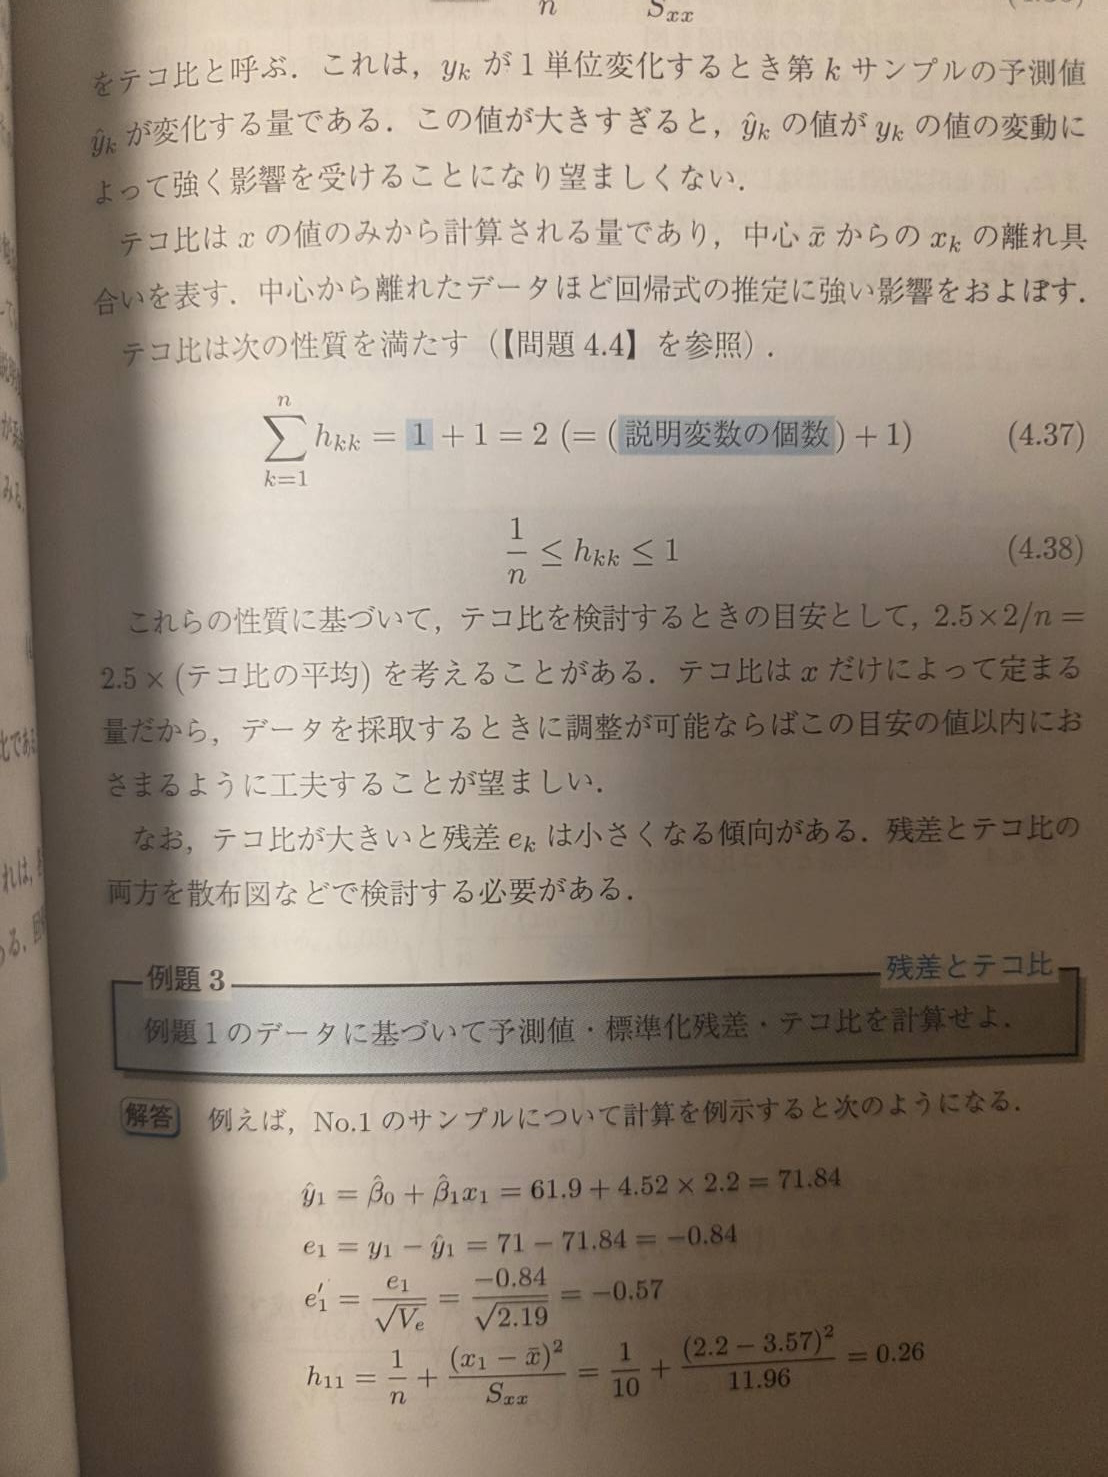
\includegraphics[width=0.8\linewidth]{image.png} % 拡張子.pngを直接指定可能
    \caption{作成したコンパイラの実行画面（またはアセンブリの出力）}
    \label{fig:execution}
\end{figure}

\end{document}